%% ===================== 1. GIỚI THIỆU =====================
\section{Giới thiệu}

\subsection{Bối cảnh}
Containerisation và Kubernetes (K8s) là nền tảng triển khai phần mềm hiện đại nhờ tính nhẹ và khả năng co giãn. Khác với máy ảo, các container trên cùng một node chia sẻ chung Linux kernel; ranh giới cô lập (isolation boundary) chỉ dựa trên các kernel primitive như namespace, cgroup, capability và seccomp. Một thoả hiệp tại một container — thông qua privilege escalation hoặc khai thác lỗ hổng kernel — có thể vượt ranh giới này để lan sang tenant khác hoặc chiếm quyền điều khiển node~\cite{crosscontainer2023,ebpfguard2026}. Trong mô hình multi-tenant, nơi các tenant không tin cậy lẫn nhau cùng tồn tại, đây là một rủi ro hệ trọng (minh hoạ ở Hình~\ref{fig:threat}).

\begin{figure}[ht]
\centering
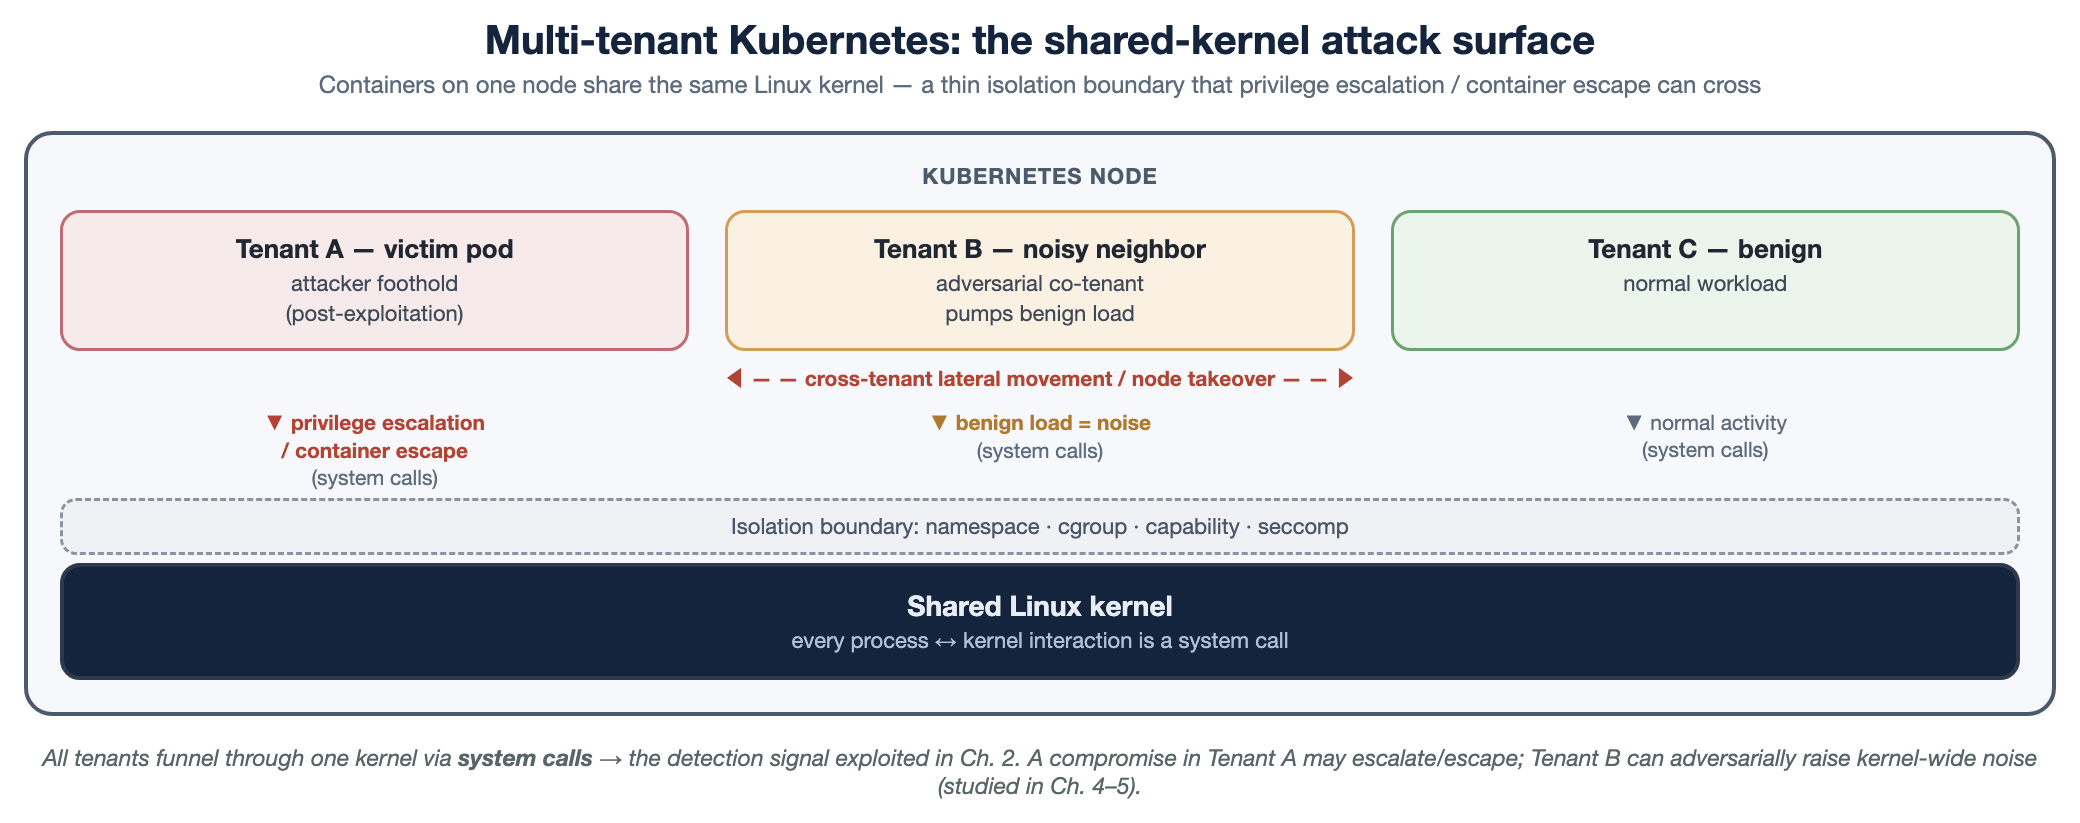
\includegraphics[width=\textwidth]{figures/fig_threat.png}
\caption{Bề mặt tấn công shared-kernel trong Multi-tenant Kubernetes.}
\label{fig:threat}
\end{figure}

Do mọi tương tác giữa tiến trình và kernel đều đi qua system call, đây là tín hiệu trung tâm của \textit{host-based intrusion detection} (HIDS — phát hiện xâm nhập trên máy chủ)~\cite{forrest1996sense,creech2014semantic,liu2018hids,bridges2019hostdata}. Công nghệ eBPF giúp thu thập system call ở mức kernel với chi phí thấp, thúc đẩy một thế hệ công cụ runtime security cho cloud-native~\cite{syairozi2025ebpfcompare,safebpf2024,hu2026eids}; trong đó \textit{DeSFAM} là một đại diện kết hợp AI mà báo cáo này lấy làm hệ cơ sở (base). Nền tảng và các công trình liên quan được trình bày chi tiết ở Chương~\ref{sec:related}.

\subsection{Động lực nghiên cứu}
DeSFAM và biến thể federated FedMon~\cite{desfam_original,fedmon2025} sử dụng cơ chế \textit{ngưỡng động} (adaptive threshold): ngưỡng cảnh báo được tự động nâng lên khi mức độ hoạt động của hệ thống gia tăng, nhằm hạn chế báo động giả phát sinh từ benign behavioral drift (sự trôi dạt hành vi lành tính theo thời gian). Mặc dù cùng hướng tới môi trường multi-tenant, cả hai chỉ được đánh giá trong điều kiện vận hành lành tính, chưa xét đến sự hiện diện của một đối thủ.

Chính cơ chế thích nghi này lại làm nảy sinh một nghịch lý an ninh. Trên hạ tầng public cloud, nơi các tenant dùng chung tài nguyên, một co-tenant không đáng tin có thể \textit{chủ động} sinh ra tải nền có mức bất thường cao — hiện tượng noisy neighbor (hàng xóm gây nhiễu) — kéo ngưỡng động lên cao hơn mức phản ánh rủi ro thực sự. Một tấn công có tín hiệu thấp (stealthy) khi đó rơi xuống dưới ngưỡng và thoát khỏi phạm vi phát hiện. Như vậy, cơ chế vốn được thiết kế để giảm báo động giả lại trở thành một attack surface (bề mặt tấn công). Mức độ nguy hiểm phụ thuộc vào một chi tiết tưởng nhỏ: ngưỡng được cập nhật \textit{vô điều kiện} (sau mọi cửa sổ) hay \textit{có điều kiện} (chỉ trên cửa sổ không bị gắn cờ) — và chính đặc tả của DeSFAM lại không nhất quán về điểm này (Mục~\ref{ss:desfam}). Báo cáo kiểm chứng trực tiếp giả thuyết này (các khoảng trống nghiên cứu tại Mục~\ref{ss:gap}).

\subsection{Câu hỏi nghiên cứu và nội dung}
Báo cáo hướng tới hai câu hỏi nghiên cứu:
\begin{description}[leftmargin=1.4cm,style=nextline]
\item[RQ1] Bộ phát hiện kiểu DeSFAM đạt năng lực phát hiện ở mức nào đối với tấn công privilege escalation (leo thang đặc quyền) và container escape (thoát container) trên dữ liệu thực, đo bằng recall, precision và AUC?
\item[RQ2] (trọng tâm) Khi ngưỡng EMA được cập nhật \textit{vô điều kiện}, một noisy neighbor bơm tải lành tính có làm nâng ngưỡng và qua đó tạo điều kiện cho evasion (né tránh phát hiện) hay không; mức độ biến thiên ra sao theo cường độ nhiễu và loại tấn công; và dạng cập nhật \textit{có điều kiện} của Algorithm 2 (DeSFAM) có loại bỏ được lỗ hổng này không?
\end{description}

Tương ứng, nội dung nghiên cứu gồm ba phần: (i) tái lập bộ phát hiện kiểu DeSFAM và đánh giá năng lực phát hiện trên tập dữ liệu thực DongTing (RQ1); (ii) phát biểu chính xác, kiểm định và định lượng giả thuyết \textit{threshold-inflation evasion} — kẻ tấn công lợi dụng việc ngưỡng động bị nâng để né tránh phát hiện — trên anomaly score thực, có kiểm định thống kê, đồng thời chỉ ra rằng dạng cập nhật \textit{vô điều kiện} tự nâng ngưỡng ngay cả khi không có đối thủ (self-inflation); và (iii) chỉ ra \textit{sự thiếu nhất quán} giữa công thức EMA (vô điều kiện) và Algorithm 2 (có điều kiện) của DeSFAM, và kiểm chứng rằng dạng cập nhật có điều kiện của Algorithm 2 vô hiệu hoá hoàn toàn vector tấn công ($0\%$) — tức là một biện pháp \textit{thiết yếu về an ninh}, không chỉ để giảm báo động giả (RQ2).

\subsection{Cấu trúc báo cáo}
Phần còn lại của báo cáo được tổ chức như sau: Mục~\ref{sec:related} — cơ sở lý thuyết và công trình liên quan; Mục~\ref{sec:method} — phương pháp luận; Mục~\ref{sec:setup} — thiết lập thực nghiệm; Mục~\ref{sec:results} — kết quả; Mục~\ref{sec:discuss} — thảo luận và threat to validity; Mục~\ref{sec:concl} — kết luận; Phụ lục~\ref{sec:repro} — hướng dẫn tái lập.
